\begin{figure}[htbp]
\centering
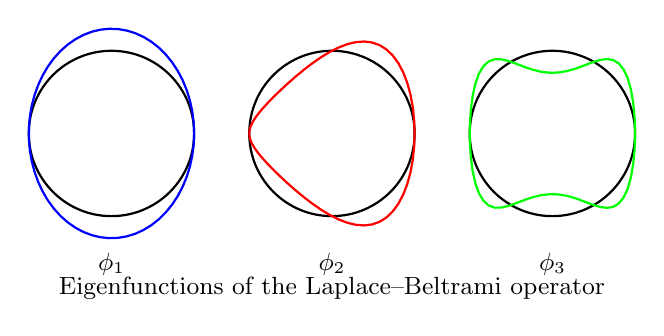
\begin{tikzpicture}[scale=0.7]
  % Eigenfunction phi_1
  \begin{scope}[xshift=0cm]
    \draw[thick] (0,0) circle (1.5);
    \draw[blue,thick,domain=0:360,samples=60] plot ({1.5*cos(\x)},{1.5*sin(\x)+0.4*sin(\x)});
    \node[below,font=\small] at (0,-2) {$\phi_1$};
  \end{scope}
  % Eigenfunction phi_2
  \begin{scope}[xshift=4cm]
    \draw[thick] (0,0) circle (1.5);
    \draw[red,thick,domain=0:360,samples=60] plot ({1.5*cos(\x)},{1.5*sin(\x)+0.4*sin(2*\x)});
    \node[below,font=\small] at (0,-2) {$\phi_2$};
  \end{scope}
  % Eigenfunction phi_3
  \begin{scope}[xshift=8cm]
    \draw[thick] (0,0) circle (1.5);
    \draw[green,thick,domain=0:360,samples=60] plot ({1.5*cos(\x)},{1.5*sin(\x)+0.4*sin(3*\x)});
    \node[below,font=\small] at (0,-2) {$\phi_3$};
  \end{scope}
  \node[font=\small] at (4,-2.8) {Eigenfunctions of the Laplace--Beltrami operator};
\end{tikzpicture}
\caption{First three eigenfunctions of the Laplacian on a circle. The eigenvalues $\lambda_k$ form the shape spectrum.}
\label{fig:shape_spectra}
\end{figure}
